\chapter{Engendering Team Code Ownership}
\label{TeamCodeOwnershipChapter}

\section{Summary}

\textit{Context:} This chapter examines team code ownership, a core category of our theory of sustainable software development presented in the previous chapter. Team code ownership is a software development practice where any team member can modify any part of the team's code. However, many factors beyond official policy affect a developer's sense of ownership. 

\textit{Objective:} The purpose is to understand the factors that affect a team's sense of code ownership.

\textit{Method:} Following Constructivist Grounded Theory, we conducted a \durationOfResearchStudyAdjective{} participant-observation of \numberOfObservedProjects{} software development projects, and interviewed \numberOfInterviews{} software engineers, interaction designers, and product managers.  When team code ownership emerged as a core category in our study, additional data was collected to investigate factors associated with perceived code ownership and related phenomena.

\textit{Results:} Team code ownership is a feeling. Developers feel team code ownership more when they understand the system context, have contributed to the code in question, perceive code quality as high, believe the product will satisfy the user needs, and perceive high team cohesion.  

\textit{Limitations:} Outcomes of grounded theory research are not statistically generalizable to defined populations, and may not apply to organizations with different software development cultures.

\textit{Conclusion:} Team code ownership is rooted in numerous cognitive, emotional, contextual and technical factors and cannot be achieved simply by policy. 

\section{Introduction}
\textit{Team Code Ownership} (which is similar to \textit{Collective Code Ownership} and \textit{Shared Code}) is a software development practice where any developer on a team has the right to change any of the team's code. Team code ownership is intended to accelerate development by allowing any developer to fix any team bug and by mitigating delays due to vacations, illness, and other absence \cite{BeckExtremeProgramming2004}.
 
While some research has investigated the effects of different code ownership models, we are unaware of any studies that specifically investigate developers' sense of team code ownership; that is, the complex interactions between developers' knowledge, emotions, and approach to code ownership.  

When team code ownership emerged as a core category of our grounded theory study, additional data was collected to investigate factors associated with perceived code ownership and related phenomena. 

Participant observation quickly revealed that having the right to change a file does not mean that a specific developer will feel empowered to and justified in making a specific change. For example, a developer may feel reluctant to change code that he or she does not really understand. As the research refined this core finding and drove further data collection, five factors affect feelings of team code ownership. 

This chapter consequently reviews existing research connected to team code ownership (Section \ref{TeamCodeOwnnershipRelatedWork}), describes some aspects of the grounded theory approach related to code ownership (Section \ref{TeamCodeOwnershipResearchMethod}), and presents the emerging results: five factors associated with team code ownership (Section \ref{TeamCodeOwnership}). Section \ref{Discussion} discusses the study's implications and limitations, followed by a summary of its contributions (Section \ref{TeamCodeOwnershipConclusion}).
\section{Related Work}
\label{TeamCodeOwnnershipRelatedWork}

\subsection{Team Code Ownership}
In Extreme Programming \cite{BeckExtremeProgramming2004}, Kent Beck describes a set of interdependent practices for managing feature development and facilitating a collaborative team environment. One of these practices is \textit{collective ownership}---\quotes{Anyone can change any piece of code in the system at any time.} \cite{BeckExtremeProgramming1999}. The book contrasts collective ownership against \quotes{no ownership} and \quotes{individual ownership.} In 2004, collective ownership is renamed \textit{shared code} \cite{BeckExtremeProgramming2004}.

In 2006, Martin Fowler defined \textit{collective code ownership}, similarly to Beck \cite{FowlerCodeOwnership}, as a contrasting team position to \quotes{strong code ownership} where each file has one owner and \quotes{weak code ownership} where developers can change files, but an owner keeps an eye on files for which they are responsible. 

Later, Bird et al. \cite{BirdDontTouchMyCode} contrasted the effects of strong- and weak-ownership. They demonstrated that weak ownership leads to more defects than strong ownership for Windows Vista and Windows 7. The study defined ownership for a software component as a percentage of the version control commits for a single developer. They defined a major contributor as someone who has more than 5\% of the git commits. A sensitivity analysis revealed that defining strong code ownership within the range from 2\% to 10\% produced similar results for the study.

Meanwhile, Murphy  \cite{MurphyIEEESoftware} argued that the concept of code ownership must be unpacked and expanded. He argued that the complexities of code ownership are missed by merely examining git commits to determine who modified which files.

This research defines \textit{team code ownership} as \quotes{the ability for any developer on a team to change any of the team's code.} For small systems and teams, \textit{collective code ownership} and \textit{team code ownership} are practically synonymous since a member of a four person team usually has the ability to modify any part of the team's code. For a large system with multiple teams, in practice, teams would have strong ownership of their portion of the system. Allowing any pair to modify any part of Microsoft Windows or Pivotal Cloud Foundry is impractical. For a large system with poorly defined team boundaries, it is possible for all the teams to adopt \textit{collective code ownership} without achieving \textit{team code ownership} as one team's changes to the code base may negatively affect other teams.

Team code ownership requires more than a team saying, \quotes{everyone can modify anything.} Instead, this research examines how a team feels that they own the code. This research defines \quotes{sense of team code ownership} as the degree to which individual members of the team feel collective ownership.  

\subsection{Psychological Ownership}
Psychological ownership refers to \quotes{the feeling of possessiveness and of being psychologically tied to an object} \cite{Pierce2001}. Targets of ownership, whether physical or immaterial, become the extension of one's self: \quotes{What is mine becomes (in my feelings) part of ME} \cite{Isaacs1933}. Ownership can be attached to a part or the whole. Psychological ownership occurs when the object becomes part of the psychological owner's identity. Psychological ownership answers the question, \quotes{What do I feel is mine?}

Changes in ownership can have strong effects on our self-identity. An increase in the number of possessions can produce positive effects \cite{Formanek1994}, while a decrease can lead to a personality shrinkage \cite{James1890}. Someone threatening a person's ownership can trigger strong emotions and responses.

Peirce \cite{Pierce2001} identifies three sources or \quotes{roots} of psychological ownership: \quotes{efficacy and effectance, self-identity, and having a place.} A major reason for possession of physical goods or abstract ideas is rooted in the innate human desire to be in control; being able to alter one's environment creates feelings of efficacy and pleasure. Ownership fulfills the need for self-identification as people define themselves, express themselves, and ensure their own survival by what they own. Ownership fulfills the need to have a place and a territory to possess. \quotes{Each motive facilitates the development of psychological ownership, rather than directly causes this state to occur.} Psychological ownership occurs with code because creating software can satisfy the desire for efficacy and effectance, self-identity, and having a place.

Peirce identifies three paths or \quotes{routes} to ownership: controlling the target, coming to intimately know the target, and investing the self into the target. With \emphasis{controlling the target}, targets that can be controlled are perceived to be part of the self.  As  individuals repeatedly exercise control of an object, eventually this leads to \quotes{feelings of ownership toward that object.} The higher the autonomy of the job task, the more likely ownership develops toward the activity. When a person has little control over an activity, psychological ownership is unlikely to develop. With \emphasis{coming to intimately know the target}, the association with the object creates feelings of ownership. One example is when a gardener feels that the garden belongs to the gardener. (This happens routinely with software developers who feel that they own part of the code base, when in reality, the company owns the software.) Feelings of ownership increase as one becomes intimately familiar with the object and associated with it. With \quotes{investing the self into the target,} people feel that they own what they create, shape or produce. Spending time, energy, and effort enables people to alter their view of themselves to include identity with the object. The more investing in the object, the stronger the psychological ownership. Nonroutine, complex jobs infuse more of individual's ideas resulting in increased ownership.

\section{Research Method}
\label{TeamCodeOwnershipResearchMethod}

The research method for this chapter is identical to the research method in Chapter \ref{SustainableSoftwareDevelopmentChapter}. When team code ownership emerged as one of the core categories of the Theory of Sustainable Software Development, additional data was collected in order to identify the factors affecting the sense of code ownership. As an example, Table \ref{TeamCodeOwnershipChainOfEvidence} presents  some quotes illustrating potential threats that can erode team code ownership for the system context factor. Section \ref{TeamCodeOwnership} introduces the factors (system context, code contribution, code quality, product fit, and team cohesion) and are the main contributions for this chapter.  

\begin{table}[t]
\renewcommand{\arraystretch}{1.5}
\centering
\caption{Examples of Threats for the System Context factor}
\label{TeamCodeOwnershipChainOfEvidence}
\begin{tabular}{|p{\twoColumnWidth{}}|}
\hline
Threat: Increasing knowledge silos  \\
\hline
Sharing knowledge around whole team is important.\\ 
\quotes{Knowledge silos are a red flag for me. For example, we have some siloing around certain parts of the app. Most of it is around the big pain points.} \\ \quotes{I feel that we don't have that context spread around fully.} \\
Hesitancy to jump onto stories without context.\\ 
\quotes{It does make me not completely comfortable to jump into stories on certain aspects of the system. If I was on a story that's going to deal with some tricky part of the system, I would want to be paired with somebody who had more traction on it.} \\
\hline
Threat: Increasing team size              \\
\hline
With a big team, keeping shared context is challenging as so much parallel work is being done. \\ 
\quotes{Having five, sometimes six pairs on the project means the team is making significant progress each week. It is hard to keep context.  If you spend a week on one part of the system, the other pairs are changing the other parts of the system. When you get back to some other place, you don't know what has changed. Because of that speed, it's harder to keep context on everything.}  \\
\hline
Threat: Increasing code base size \\
\hline
Code continues to expand.\\
\quotes{The code is complicated. It keeps on expanding. It is hard to keep it all in my head. It is like the big bang, where it starts out very small and now it just keeps expanding and growing. We are still adding a bunch of features.}  \\
\hline
\end{tabular}
\end{table}


% Following Charmaz' approach to Grounded Theory \cite{Charmaz}, this research used two primary data sources: field notes collected during continuous participant observations of a 7.5-month project and interviews with \numberOfInterviews{} Pivotal software engineers, interaction designers, and product managers. The initial core question was: \quotes{What is happening at Pivotal when it comes to software development?} This question led to the Theory of Sustainable Software Development presented in Chapter \ref{SustainableSoftwareDevelopmentChapter}. When team code ownership emerged as one of the core categories of the theory, additional data was collected in order to identify the factors affecting the sense of code ownership. The factors are introduced in Section \ref{TeamCodeOwnership} and are the main contributions for this chapter.

%\subsection{Data Collection}
% The primary researcher relied on \quotes{intensive interviews,} which Charmaz summarizes as \quotes{open-ended yet directed, shaped yet emergent, and paced yet unrestricted} \cite{Charmaz}. The technique relies on open-ended questions. The purpose is for the researcher to enter into the participant's personal perspective within the context of the research question. 

% While exploring new emergent core categories, whenever possible, the researcher initiated subsequent interviews with a goal of not forcing the issue. For example, \quotes{please draw your feelings about the code} often resulted in conversations about code ownership. After the interview, the interview was transcribed into a Word document with timecode stamps for each segment.

% The primary researcher collected field notes while working as an engineer. The field notes comprise multiple paragraph entries recorded several times a week collected over a six month period. The notes describe individual and collective actions, captures what participants defined as interesting or problematic, and include anecdotes and observations. 

% \subsection{Research Context: Pivotal}
% \label{TeamCodeOwnnershipResearchContext}
% Pivotal is a large American company with 16 offices around the world. One of its divisions is Pivotal Labs. Pivotal Labs' mission is to both deliver highly-crafted software products and provide a transformative experience for their client's engineering cultures. To change a developer's way of working, Pivotal combines the client's software engineers with Pivotal's engineers at a Pivotal office where they can experience Extreme Programming in an environment conducive for agile development. % Tmp for 6 pages    For startups, Pivotal might be the first engineers working on the project. For enterprise clients, Pivotal provides additional engineering resources to accomplish new business goals. 

% A common team size is six developers plus an interaction designer and a product manager. In the history of the Palo Alto office, the number of developers on a project ranges from 2 to 28. Larger projects are organized into smaller coordinating teams with one product manager per team and one or two interaction designers per team.

% Tmp to fit in 6 pages
%Commonly utilized technologies include Angular, Android, Backbone, iOS, Java, Rails, React, and Spring which are often deployed onto Pivotal's Cloud Foundry. 

% Pivotal Labs has followed Extreme Programming \cite{BeckExtremeProgramming2004} since the late 1990s. While each team is autonomous in making its own decisions as to what is best for a particular project, the company culture strongly suggests following all of the core practices of Extreme Programming. % Tmp to fit in 6 pages  This includes Pair Programming, Test Driven Development, Weekly Retrospectives, Daily Stand-ups, Prioritized Backlog, Whole Team ownership of the project and code base, plus Kanban's notion of work flowing through people.

\section{Team Code Ownership}
\label{TeamCodeOwnership}

In the literature, collective code ownership is often treated as a policy statement. In this case, simply claiming that \quotes{anyone can modify any piece the code} was not sufficient to engender willingness to modify any file. Rather, ownership is an emotional or qualitative attribute that ties all developers on the team to the project and code base. It is a spectrum where, on one side, each individual has ownership of only their code, and on the other side, everyone on the team owns the entire code base. Some events appear to erode the team's sense of ownership over the project's duration, while some practices appear to counteract these erosions. This section details the five factors that appear most related to team code ownership and examples of events or tendencies that erode it. 

\subsection{System Context}
\textbf{Definition:} System context is the knowledge and situational awareness about the code, including the discourse that surrounds the code. System context includes understanding existing design decisions, underlying technologies, the relationship between features and user needs, and the implementation of existing features.

\textbf{Purpose:} Developing an in-depth knowledge of the system exercises the \quotes{intimately knowing the target} path of psychological ownership.

For a pair to work efficiently on any part of the system, one of them needs to have enough context to know how that part of the system works. Without enough context, a pair might struggle, slow down, or be blocked in working on a feature.

Team code ownership seems to vary with the context that the developer has about the code; the more the developer knows, the higher the sense of ownership. Knowledge silos, the size of the code base, or the number of developers working in parallel can make it difficult for a programmer to develop a deep system context level.

\textbf{Threat: Increasing knowledge silos.} When developers routinely work on one part of the code base, they can develop specific system context not shared by the team. Code specialization impedes anyone on the team from modifying any part of the team's code.  One team said \participantQuote{we need Marion on that story, only she knows the Apple watch code base,} and \participantQuote{Shea knows the ins-and-outs of the legacy integration, we need him to work on this story,} which means there is a hindering imbalance between the individual and team understanding of the code.

% \textbf{Threat: Increasing code base size.} One team started working with a large code base that was over eight years old and the team did not have a full understanding of the system. Initially, the team felt little ownership of the code, even though the team was responsible for it and agreed to \singleQuote{team code ownership.} Often the team would need to ask a product manager why certain features exist in the code to understand the code's purpose and implementation. In time, as the team worked with the code and gained context, the team's sense of ownership improved.

\textbf{Threat: Increasing team size.} We observed the relationship between team size and code context on \numberOfObservedProjects{} Pivotal projects as a participant-observer. As team size increases, the ability to gain system context decreases. Every day, all pairs are adding to the system. On a five pair team, so much work is happening each day that it becomes increasingly difficult to keep track of everything that changes.

One developer on a ten-person project said, \participantQuote{I feel that we don't have the context spread around fully. Having five, sometimes six, pairs on the project makes it go really fast, so it's hard to keep context.}

When developers do not have context about part of a system, or context about what remains to be done to finish a story, reluctance to start the next story at the top of the backlog emerges. It's easier to start a story that touches part of the system that they know. As one developer reflected, \participantQuote{I am not entirely comfortable to jump into stories on certain aspects [of the system].}

As a coping strategy, one developer, before the start of the work day, skimmed the git commits from the previous day to learn about new classes and changes in design and to understand the features the team added. 

As team size grows, there is a potential risk of decreasing an individual developer's sense of team code ownership. 

\subsection{Code Contribution}
\textbf{Definition:} Code contribution is the portion of the code that a given developer has worked on. 

\textbf{Purpose:} Personally contributing to the code base increases a developer's sense of ownership by exercising \quotes{investing in the target} path of psychological ownership. 

As a developer works on the code base, the developer's system context level increases. While code contribution level influences the system context level, it is not necessary related: developers might learn about the code through other means different from direct contribution, including conversations at stand-up, impromptu team huddles, or a pair saying \participantQuote{check out what we did yesterday.}

\textbf{Threat: Inability to contribute.}  A developer's inability to contribute to the code base decreases the developer's sense of ownership. 

This could happen, for instance, during a pair programming breakdown. When the pairing experience breaks down, one person drives the code development while the partner passively watches. (\quotes{Performance Pair Programming} describes when one developer plows through a story and stops listening to the developer's partner.)  When one person is writing all the code, individual code ownership replaces team code ownership.  

%six paper vesion
In one situation, the partner took over and ignored the participant's input. The participant reflected, \participantQuote{I would not be able to explain deeply what we had done. I would not be able to maintain it. I didn't really write it, so I feel very little ownership of it.} 

% full version: In one situation, the partner took over and ignored the participant's input. The participant reflected, \participantQuote{I did not understand what was really going on. I wouldn't be able to explain deeply what we had done. I wouldn't be able to maintain it. I didn't really write it, so I feel very little ownership of it.} 


Ideally, Pair Programming is a collaborative experience where both individuals are unable to tell who wrote which portions of the code. 

\subsection{Code Quality}
\textbf{Definition:} Code quality relates to how well the code satisfies the project's desirable quality attributes. Desirable quality attributes might include design qualities, performance, reliability, scalability, security,  testability, and usability \cite{Meier2009}. 

\textbf{Purpose:} A high quality product satisfies the self-identity motivation of psychological ownership. Developers might not want to be identified with a low quality product.

Low-quality products also tend to involve a disproportionate amount of bug fixes. Developers need a balance between creating new features and fixing bugs each week. Working only on bugs for weeks affects their sense of ownership.    

\textbf{Threat: Pressure to deliver and deprioritizing continuous refactoring.} When developers are pressured to deliver more features at the expense of Continuous Refactoring, the code acquires technical debt, the code becomes more difficult to work with, and developers can begin to feel indifferent about the code. When developers begin to experience code apathy, this decreases their sense of team code ownership. 

When the team neglects refactoring, new code is simply bolted onto the existing design. Each time the team bolts something else on, bolting on the next piece becomes more complicated. Thus, a dilemma arises for the programmers working on the next story that touches this part of the code: do they continue bolting on more code, or do they perform the pretermitted refactoring? A team's avoidance of refactoring may be a sign that code apathy is settling in. Code apathy results in reduced quality, as the developers become less invested in the craftsmanship of the code.

One developer felt \participantQuote{proud and disgusted} about the code base. He is simultaneously proud of each refactoring that the team performed and disgusted by the technical debt the team accrued by taking shortcuts to ship more features. The developer drew Figure \ref{Programmer1} to show his feeling about the code, \participantQuote{it is generally orderly with a few bits that maybe are not as orderly.}

Before the first launch of a product, the product manager suggested that the team deliver more features at the expense of technical debt. For some of the team, this was an unacceptable tradeoff, and those developers decided not to cut corners. Others on the team complied with the request and incurred technical debt. The entire team ended up paying the consequences with extensive refactors after the launch. On a communal code base, one pair adding tech debt affects everyone on the team.

When code apathy settles in, team members adopt the attitude that someone else will solve the problem with the code. When this attitude permeates a team, no one is solving the problems. 

\begin{figure}[t]
\centering
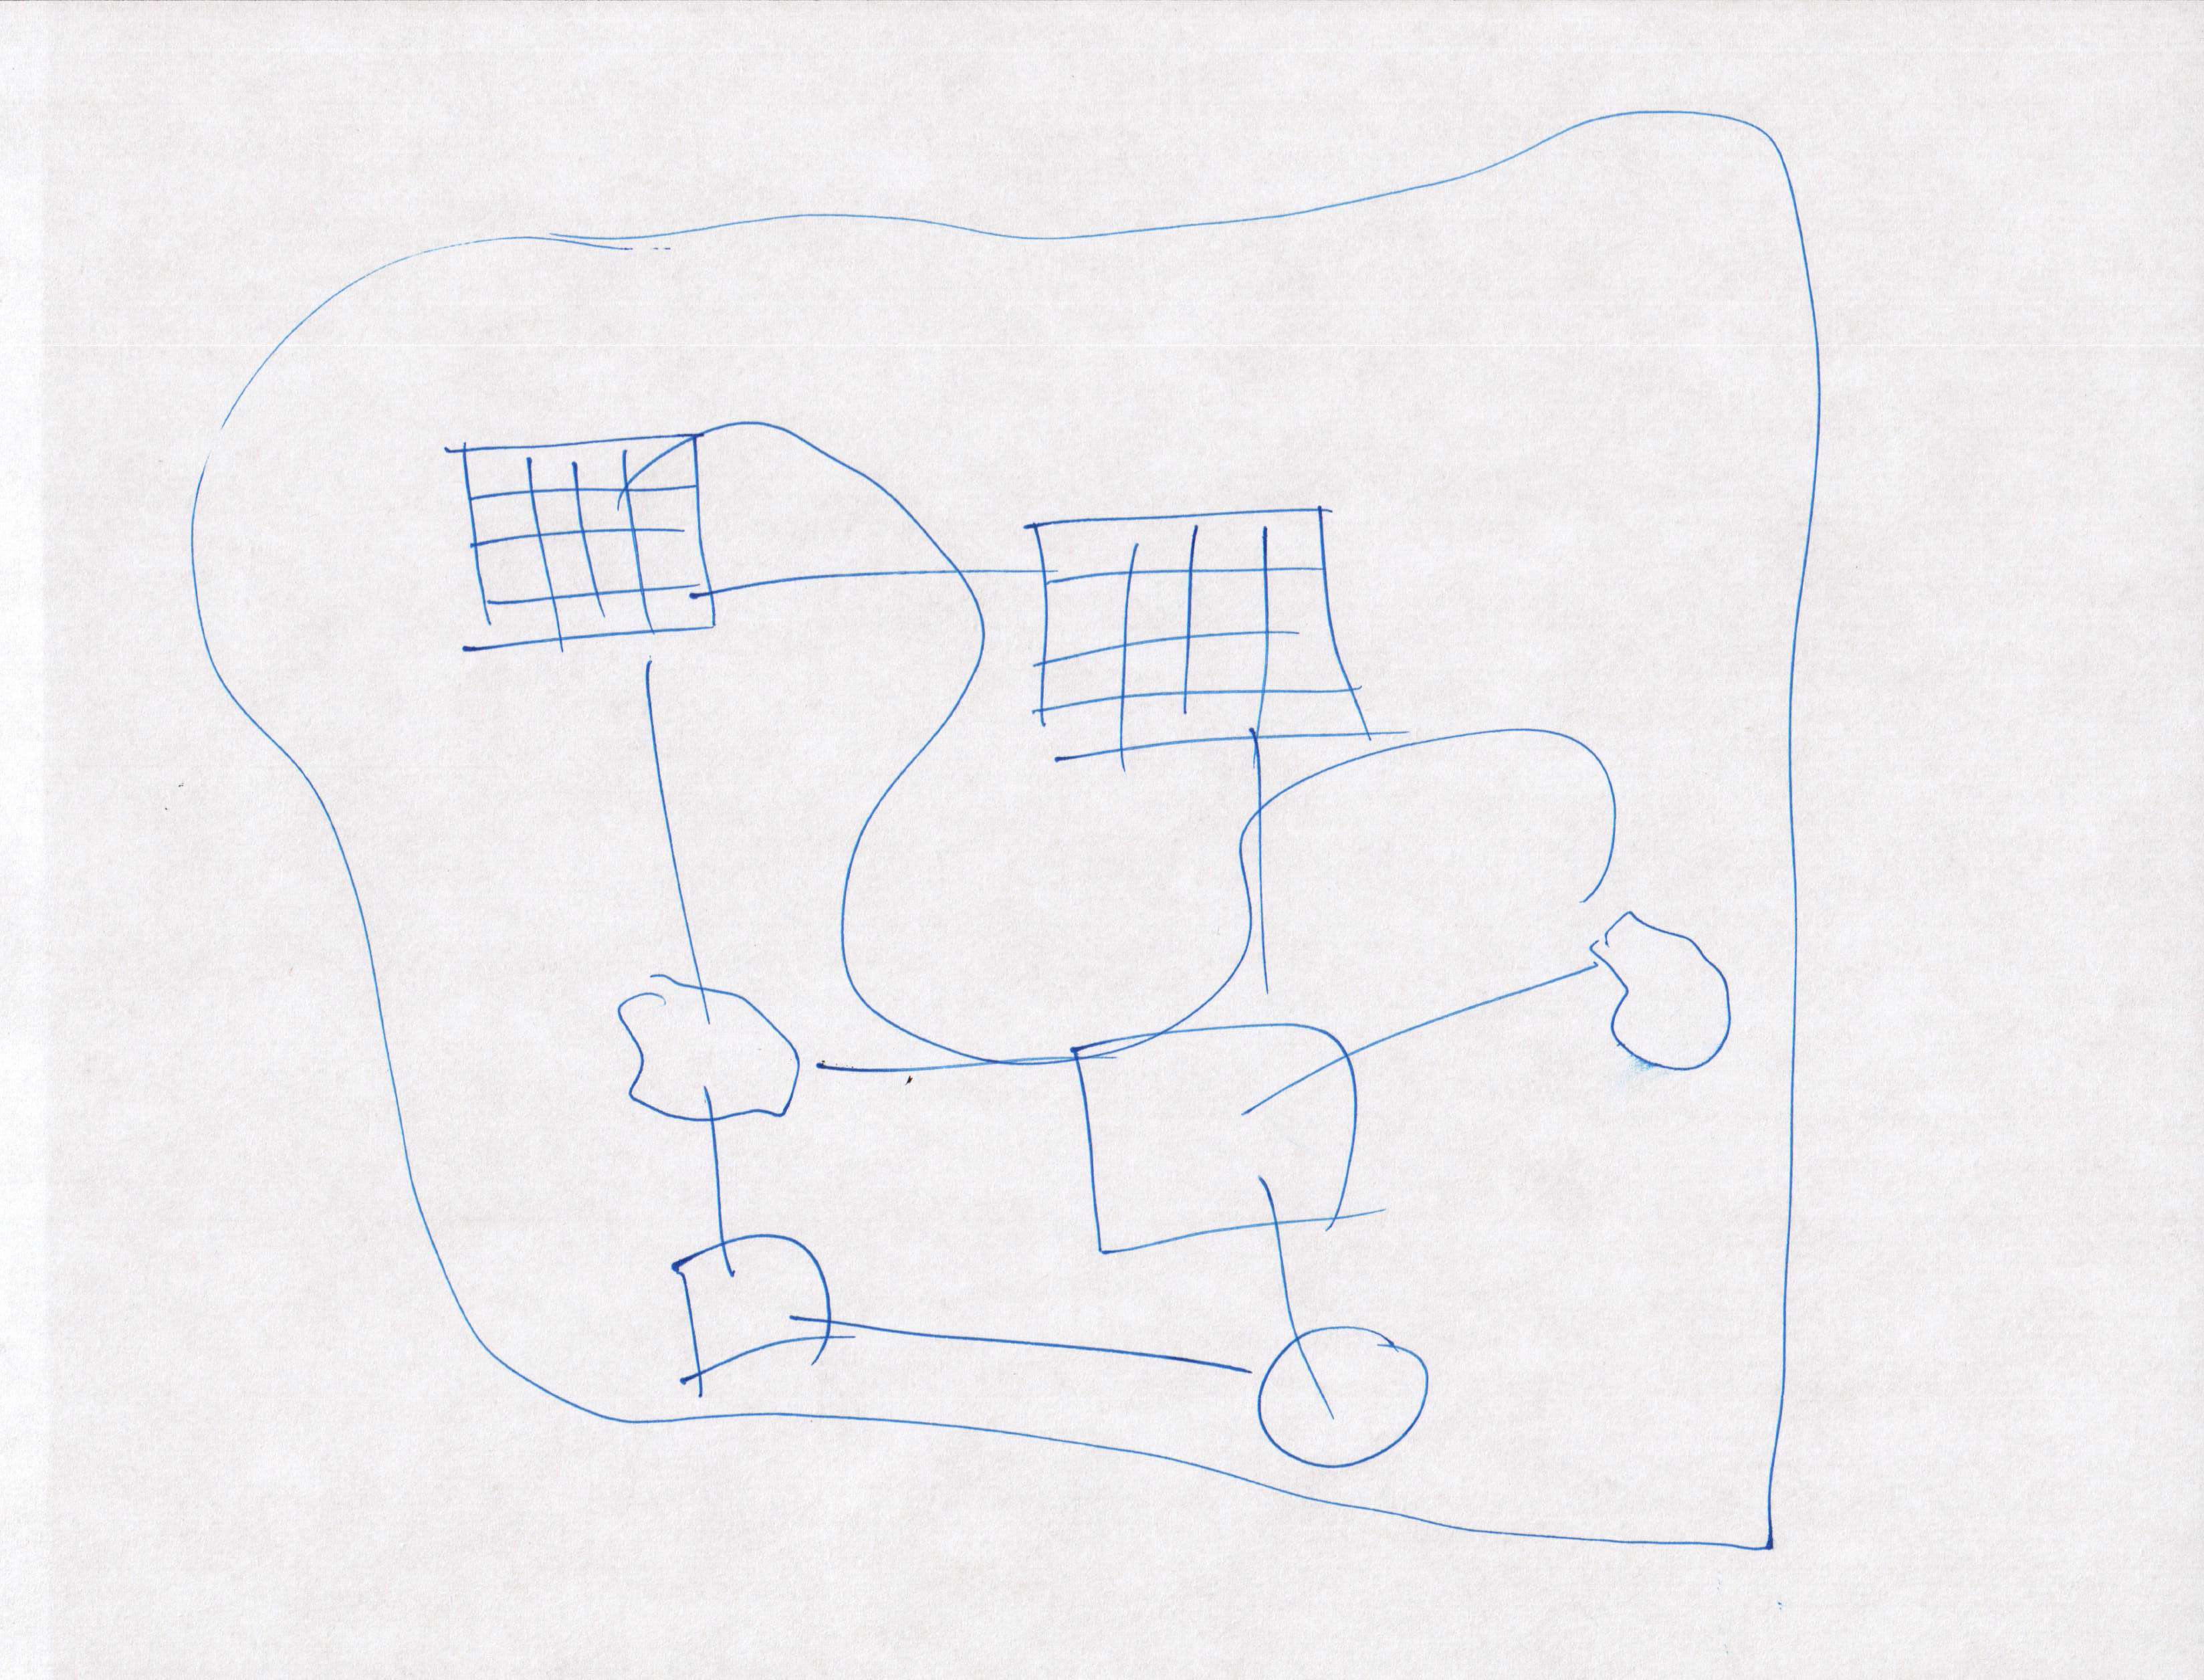
\includegraphics[width=3.45in]{team_code_ownership_images/CodeOwnership.jpg}
\caption{\quotes{Draw how you feel about the code}}
\label{Programmer1}
\end{figure}

The team wants to feel pride in improving code quality.  It feels good to be improving the code design and readability. If the team starts neglecting these concerns, it can engender a sense of disgust and apathy for the code can spread throughout the team.

\subsection{Product Fit}
\textbf{Definition:} Product fit is developers believing that features of the product will satisfy the user's needs.

\textbf{Purpose:} The observed engineers want to create products that matter to the users. Delivering a product that matters to someone satisfies the self-identity motivation of psychological ownership.

\textbf{Threat: Ignoring user feedback.} When the product manager ignores feedback from user research and usability testing, developers may lose faith in the product's ability to achieve its goals. Developer motivation and engagement can decrease when developers perceive they are building a feature that users have explicitly said they do not want yet is built to solve a business goal. 

\textbf{Threat: Ignoring developers feedback about the product.} Pivotal's balanced team approach is founded on collaboration between product managers, interaction designers, and developers. When product managers or other stakeholders ignore feedback from developers, developers can begin to feel less ownership in the product, and in turn, be less motivated to work on the project. 

%When picking up a story, a developer verifies that the story contains clear acceptance criteria. In the absence of acceptance criteria, the developer typically clarifies what needs to be done with the product manager. On one project during which the stakeholders ignored feedback from the developers, one developer recalled, \participantQuote{In this case, I don't feel like spending the extra energy to go and say, `Hey, are you sure? Is this what you want?'} 

Feature apathy or product apathy can result in a poorly crafted product that does not meet the customer's needs.

\subsection{Team Cohesion}
\textbf{Definition:} Team cohesion is the degree to which team members identify as part of the team, stick together through adversity and take pride in the team's accomplishments \cite{Bollen1990Perceived, Beal2003Cohesion, Whitworth2007Motivation}.

\textbf{Purpose:} Team cohesion satisfies the \quotes{having a place} motivation of psychological ownership.

\textbf{Threat: Distancing a developer from the team.} Team apathy manifests when developers do not feel that they are a part of the team. Developers feel less ownership of the code base when they feel excluded from the team.

Several behaviors were observed that can distance a developer from the team: interrupting the developer during discussions, using poor listening skills so that the developer feels unheard, or talking beyond the developer's level of technical expertise. 

On one team, during discussions, the team talked about code but never looked at the source code. One developer found these abstract discussions difficult to follow. Sometimes the team discussed parts of the code that the individual had not seen recently. When the team discussed two variants of coding practices without showing concrete examples, the programmer could not contribute. When the developer raised this issue to the team and the team continued with the status quo, the programmer felt marginalized by the team.

Poor onboarding of developers can contribute to feelings of isolation. On one project, there was a time crunch and the team was feeling the pressure to deliver stories. When the team added developers, the team had a \quotes{sink or swim} attitude, letting new team members figure things out on their own, hence making them feel unwelcome.

When developers feel that the team does not care about them, their sense of ownership can decrease.

\section{Discussion}
\label{Discussion}
\subsection{Transitioning to team code ownership}
\label{Transitioning}

The above results have numerous implications for teams attempting to transition to team code ownership. Some developers effortlessly make the transition to team code ownership. They immediately see the benefits of being able to modify any part of the code base and quickly shift from \quotes{I made this} (personal ownership) to \quotes{we made this} (collective ownership.)

Others may struggle with team code ownership for several reasons:

\begin{itemize}  

\item Developers may struggle to transition to a caretaker mindset.  In one interview, a software engineer struggled to describe the developer's relationship with the code on a very challenging project and settled in on the caretaker metaphor: \participantQuote{Sometimes I kind of feel like a janitor to [the code base].  Maybe caretaker would be better. Yeah, probably caretaker. I feel like a janitor just cleans up messes, but a caretaker makes things better.} 

\item A developer may be distraught at \participantQuote{seeing my work slowly removed from the app.} 

\item Developers can no longer take pride in functionality that they exclusively develop.

\item Existing knowledge silos, which hinder team code ownership, may be slow to break down.
 
\end{itemize}

New hires struggling with the transition slowly realize that \participantQuote{someone else is going to take over and they're going to do fine. I can move onto something else and that's okay.} They recognize the lack of long-term individual authorship, learn to expect their code to be transitory, develop trust in their teammates and thus loosely hold personal contributions. \participantQuote{The code that I write today may be in the code base for a little while, and it will evolve into something better.} Eventually,  they experience the benefits of a collaborative environment: \participantQuote{People are a lot more flexible all across the board, with changing things or accepting feedback or collaborating,} and the team can say \participantQuote{Hey, this is our code!}

Shifting from individual to team code ownership may require multiple and complementary practices to actively remove knowledge silos. In this case, daily pair rotation helped combat knowledge silos. Moreover, for developers with strong individual ownership tendencies, sharing ownership first with a small group (where trust and communication come easier) may help. One Pivotal engineer uses improvisation and collaboration games to help teams practice letting go of control, trusting the team, and learning to be pleasantly surprised by what emerges. 

\subsection{Results Evaluation}

The factors influencing team code ownership presented in Section \ref{TeamCodeOwnership}, have emerged from the Grounded Theory research study introduced in Section \ref{SustainableSoftwareDevelopmentTheory}. While other factors may influence team code ownership, this discussion focuses only on those that were observed during the study. Grounded Theory studies can be evaluated using the following criteria \cite{Charmaz}: 

\textbf{Credibility:}  The \numberOfInterviews{} intensive open-ended interviews and numerous field notes from participant-observation serve as a rich and credible data set for the analysis. 

\textbf{Originality:} The research broadens the idea of team code ownership by acknowledging that collective code ownership is more than a policy statement, and by uniquely identifying factors that affect the team's sense of code ownership.

\textbf{Resonance:} Several participants reviewed the findings and indicated that both the factors and threats resonate with their experience.

\textbf{Usefulness:} The study identifies factors associated with ownership and suggests several ways of engendering team code ownership.

This work analyzed software projects at the Silicon Valley office of Pivotal following Extreme Programming. From an \textbf{external validity} perspective, grounded theory is non-statistical, non-sampling research. The results therefore cannot be statistically generalized to a population. Rather, researchers and professionals can adapt the concepts and ideas to other contexts case-by-case. 

Finally, the results might be influenced by \textbf{researcher bias} or \textbf{prior knowledge bias}. A risk of the participant-observer technique is that the researcher may lose perspective and become biased by being a member of the team. While a participant-observer gains perspective an outsider cannot, an outside observer might see something a participant observer will miss. Similarly, while prior knowledge helps the researcher interpret events and select lines of inquiry, prior knowledge may also blind the researcher to alternative explanations \cite{GlaserIssues}. These risks were mitigated by recording interviews and having the other researchers review the coding process. 

\section{Conclusion}
\label{TeamCodeOwnershipConclusion}
This chapter reports results from a participant-observation, constructivist grounded theory study at Pivotal, a large American software company employing Extreme Programming practices. It provides three main contributions.

1) The observations clearly indicate that \textbf{team code ownership is a feeling to be engendered not a policy to be decreed}.

2) Meanwhile, both discussions with and observations of participants suggest five factors associated with strong feelings team code ownership. Pivotal developers more acutely feel team code ownership when i) they understand the system context; ii) they have contributed to the code in question; iii) they perceive code quality as high; iv) they believe the product will satisfy user needs; and v) they perceive team cohesion as high.   

3) Moreover, diverse events and trends can undermine sense of ownership, including:  increasing knowledge silos, increasing code base size, increasing team size, inability to contribute, pressure to deliver and deprioritizing continuous refactoring, ignoring user feedback, ignoring developer feedback, and distancing a developer from the team. 

In conclusion, Pivotal's developers find team code ownership highly advantageous; however, transitioning to a team code ownership model is easier for some than others. Some agile practices including continuous pair programming, overlapping pair rotation, continuous refactoring, and test driven development appear to help. Promising angles for future research include more nuanced explorations of the code ownership spectrum, further exploration of the roles of emotion and identity, as well as developing specific practices for facilitating ownership transitions. 



